% This is "sig-alternate.tex" V1.9 April 2009
% This file should be compiled with V2.4 of "sig-alternate.cls" April 2009
%
% This example file demonstrates the use of the 'sig-alternate.cls'
% V2.4 LaTeX2e document class file. It is for those submitting
% articles to ACM Conference Proceedings WHO DO NOT WISH TO
% STRICTLY ADHERE TO THE SIGS (PUBS-BOARD-ENDORSED) STYLE.
% The 'sig-alternate.cls' file will produce a similar-looking,
% albeit, 'tighter' paper resulting in, invariably, fewer pages.
%
% ----------------------------------------------------------------------------------------------------------------
% This .tex file (and associated .cls V2.4) produces:
%       1) The Permission Statement
%       2) The Conference (location) Info information
%       3) The Copyright Line with ACM data
%       4) NO page numbers
%
% as against the acm_proc_article-sp.cls file which
% DOES NOT produce 1) thru' 3) above.
%
% Using 'sig-alternate.cls' you have control, however, from within
% the source .tex file, over both the CopyrightYear
% (defaulted to 200X) and the ACM Copyright Data
% (defaulted to X-XXXXX-XX-X/XX/XX).
% e.g.
% \CopyrightYear{2007} will cause 2007 to appear in the copyright line.
% \crdata{0-12345-67-8/90/12} will cause 0-12345-67-8/90/12 to appear in the copyright line.
%
% ---------------------------------------------------------------------------------------------------------------
% This .tex source is an example which *does* use
% the .bib file (from which the .bbl file % is produced).
% REMEMBER HOWEVER: After having produced the .bbl file,
% and prior to final submission, you *NEED* to 'insert'
% your .bbl file into your source .tex file so as to provide
% ONE 'self-contained' source file.
%
% ================= IF YOU HAVE QUESTIONS =======================
% Questions regarding the SIGS styles, SIGS policies and
% procedures, Conferences etc. should be sent to
% Adrienne Griscti (griscti@acm.org)
%
% Technical questions _only_ to
% Gerald Murray (murray@hq.acm.org)
% ===============================================================
%
% For tracking purposes - this is V1.9 - April 2009

\documentclass{sig-alternate}
  \pdfpagewidth=8.5truein
  \pdfpageheight=11truein

\begin{document}
%
% --- Author Metadata here ---
\conferenceinfo{Machine Learning Course}{June, 2015, Shanghai, China.}
\CopyrightYear{2015} % Allows default copyright year (2002) to be over-ridden - IF NEED BE.
\crdata{}  % Allows default copyright data (X-XXXXX-XX-X/XX/XX) to be over-ridden.
% --- End of Author Metadata ---

\title{Native or Not? A Machine Learning Solution towards Judging A Person's Native Language}
%
% You need the command \numberofauthors to handle the 'placement
% and alignment' of the authors beneath the title.
%
% For aesthetic reasons, we recommend 'three authors at a time'
% i.e. three 'name/affiliation blocks' be placed beneath the title.
%
% NOTE: You are NOT restricted in how many 'rows' of
% "name/affiliations" may appear. We just ask that you restrict
% the number of 'columns' to three.
%
% Because of the available 'opening page real-estate'
% we ask you to refrain from putting more than six authors
% (two rows with three columns) beneath the article title.
% More than six makes the first-page appear very cluttered indeed.
%
% Use the \alignauthor commands to handle the names
% and affiliations for an 'aesthetic maximum' of six authors.
% Add names, affiliations, addresses for
% the seventh etc. author(s) as the argument for the
% \additionalauthors command.
% These 'additional authors' will be output/set for you
% without further effort on your part as the last section in
% the body of your article BEFORE References or any Appendices.

\numberofauthors{1} %  in this sample file, there are a *total*
% of EIGHT authors. SIX appear on the 'first-page' (for formatting
% reasons) and the remaining two appear in the \additionalauthors section.
%
\author{
% You can go ahead and credit any number of authors here,
% e.g. one 'row of three' or two rows (consisting of one row of three
% and a second row of one, two or three).
%
% The command \alignauthor (no curly braces needed) should
% precede each author name, affiliation/snail-mail address and
% e-mail address. Additionally, tag each line of
% affiliation/address with \affaddr, and tag the
% e-mail address with \email.
%
% 1st. author
\alignauthor Zhaowei Tan\titlenote{This author is the
one who did all the really hard work. All the codes, methods and approaches are written or designed by the author and his teammates (they formed the group who came up with this topic). I will EXPLICITLY POINT OUT when some work mentioned in the paper is not done by this author.}\\
       \affaddr{5120309701}\\
       \affaddr{IEEE Honor Class}\\
       \affaddr{Shanghai Jiao Tong University}\\
       \affaddr{Shanghai, China}\\
       \email{tanzw94@gmail.com}
}
% There's nothing stopping you putting the seventh, eighth, etc.
% author on the opening page (as the 'third row') but we ask,
% for aesthetic reasons that you place these 'additional authors'
% in the \additional authors block, viz.

\date{30 July 1999}
% Just remember to make sure that the TOTAL number of authors
% is the number that will appear on the first page PLUS the
% number that will appear in the \additionalauthors section.


\maketitle
\begin{abstract}
Machine learning is one of the most popular and cutting edge topics nowadays. Researchers delve into machine learning methods and models, while using this technology to solve many real world problems. Speech recognition is among the most active problems using machine learning. In this paper, I try to solve a real world speech recognition problem using machine learning. Given a audio recording with known content, I tried to figure out the identity of the speaker--a native English speaker or not. I present the process of acquiring the data, ordering the data and processing the data. After that, I use the well-structured data to learn the model with two machine learning methods, Logistic Regression and K-means, and then compare them afterwards. The experiments show that my methods can reach a maximum accuracy of 87.5\%. At the end of the paper, I provide some insights of further improving the performance.
\end{abstract}



\keywords{Machine Learning, Binary Classification, Speech Recognition}

\section{Introduction}\footnote{\\ ********************IMPORTANT********************  Dear TA, some of my sentences here will seem familiar to you because it was I that mainly wrote the manual for anyone who wanted to do our project. So I claim the copyright of that document and hence simply reuse some of the words in that manual.}
Many of us will apply for graduate schools in the near future. TOEFL score is indispensable for this process, and a higher score may increase your chances of being admitted. However, Chinese students tend to earn a low score in Speaking Task, which prohibits some top students from reaching the minimum requirements of their dream schools.

It is from this point that our team developed our idea. We aim to build a system, via machine learning methods, to help us train the accent in order to achieve a higher TOEFL score. Considering that this goal is way too far from us, we start from a simple task, judging whether a piece of a recording is from a native speaker or not.

The presented problem is in the field of speech recognition, which is among the hottest research areas in computer science field. Actually this is what our Dear Professors are currently working on. The speech recognition problems are rather hard, while some mature tools and methods have already been greatly developed.

I took advantage of several speech recognition tools, as well as built-in machine learning libraries, to swiftly solve the problem with a decent accuracy. Unlike other two available projects, a considerable part of my work is the data processing.

The paper is organized as follows. I give the sound description of the problem in Section 2. In Section 3, I present the process from which I get the data and process the data. In Section 4, multiple machine learning methods are proposed to solve the problem using the data we get. All the experimental results are shown in Section 5, after which I make discussions on the performance and elaborate possible future work in Section 6. Finally, I conclude this paper in Section 7.



\section{Problem Description}
The basic goal is a binary classification problem:
\begin{quote}\emph{
	Given a recording of a fixed script of English words, we would like to predict whether the speaker is a native English speaker or not.}
\end{quote}

Thus, given a unlabelled new data, I try to get as high a accuracy as problem. More specifically, we now possess a dataset $[X,Y]$. $X=[x_{1}^{T},x_{2}^{T},...,x_{n}^{T}]^{T}$, where $x_i$ is a recording from user $i$, speaking a given record. $Y=[y_1,y_2,...,y_n]^T$, where $y_i=1$ indicates that recording $i$ is from a native speaker while $y_i=0$ indicates that recording $i$ is from a non-native speaker (mandarin speaker in my case). I try to learn a model out of this dataset and use the model to predict whether a new recording belongs to a native, or a non-native speaker.

As we can imagine, this function will vastly benefit English as a Second Language students and teachers, people who need to learn an accent, linguists who do research in this area and all the hosts whose services differ due to native language.




\section{Data Acquisition and Processing}
After I have defined the scope of this paper and the specific problem description, it is high time that I introduced the approach to get the data and handle the data. Actually, this is the most difficult and arduous part in the whole project, because for other tasks we can utilize the existing toolkits.

In this section, I will go step by step, from getting data to handling the data, to illustrate the process of acquiring the information from scratch.
\subsection{Data Crawling}
Although the crawler has been provided in the FTP, I reiterate the issue here because I was the author of the crawler so hence I claim the authorship here. I use the crawler to crawl the data from the George Mason University Department of English Speech Accent Archive\cite{accent}. I do not own the data, and do not use the data for business purpose. All the credits of the data go to that university entity.

When writing the crawler, I used a open source python library, beautifulsoap\cite{bs}, to parse the web pages and get the intended data.

\subsection{The Description of the Data}
In the website, all the recordings are classified according to the speakers' native languages.

I now have crawled the recordings of two categories, \emph{English} and \emph{Mandarin}, combing 620 clips together. In each recording, every speaker will read the same English script:
\begin{quote}\emph{
Please call Stella. Ask her to bring these things with her from the store: Six spoons of fresh snow peas, five thick slabs of blue cheese, and maybe a snack for her brother Bob. We also need a small plastic snake and a big toy frog for the kids. She can scoop these things into three red bags, and we will go meet her Wednesday at the train station.}
\end{quote}

In addition to the recording, I scrap the basic information of the speaking, including the native language, birth place (pinpointed to the province), other language spoken, age, sex, age of starting learning English, learning method, English residence (if has, the length of the residence). These data are collected into csv files which have been provided together with the recordings.

A brief summary of the data can be found in the Table 1.

\begin{table}[ht]
\centering
\caption{Data Description}
\begin{tabular}{|c|c|c|} \hline
&Mandarin&English\\ \hline
\# of clips&561 &59 \\ \hline
\# of features&11 &11 \\ \hline

\end{tabular}
\end{table}

\subsection{Data Conversion}
MATLAB and other program languages that are able to process audio prefer .wav than .mp3. Since the data we crawled were in .mp3 format, the data conversion is indispensable. Before I realize the MATLAB is really prompt to realize this, I used a free software on MacOS, MediaHuman Audio Converter\cite{convert} to realize this. Thus I was able to convert all my raw data to .wav format.


\subsection{MAUS Implementation}
Since the audio are all about a same given paragraph, I utilized The Munich Automatic Segmentation System (MAUS)\cite{maus} to segment the audio into pieces according to each word. This is an open source free software, which can take two inputs: audio and corresponding text, and output the audio segment corresponding to each word.\footnote{This function I use is MAUSBasic, actually it contains more advanced services, by which can make the training performance better.}

This seemingly simple task is an real nightmare. Installing MAUS locally on the laptop is complicated and exhausting, which made me give up halfway.\footnote{My roommate, Lihang, actually took about a whole day to make that working.} As a result, i took advantage of the MAUS Webservices instead. Nevertheless this was still an exhausting which took me hours. \footnote{Sadly, this is proved to be useless effort in the end because my teammate, Zhichen, told me that WebMAUS, a MAUS service with interface can provide a easier interface of MAUS.}

The alternative way I took is to write a PHP file to call the interface of MAUS Webservices. Figure 1 is a sample curl command to call the service, which will upload english1.wav to the server and run MAUSBasic online.


\begin{figure}
\centering
\fbox{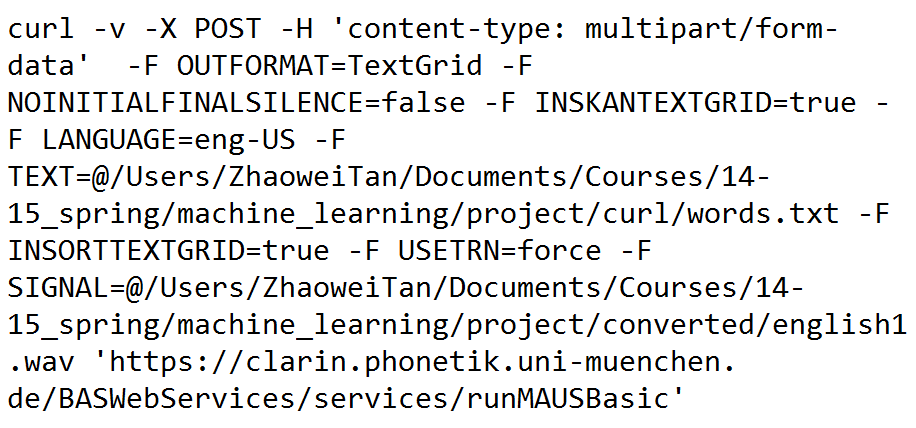
\includegraphics[scale = 0.35]{code.png}}
\caption{A sample curl script to call MAUS.}
\end{figure}

Thus, I took advantage of PHP curl and write a PHP script to recursively upload my converted .wav file, let the server do the MAUS things and then fetch the output Textgrid. After having the given TextGrid, thanks to Jiaming, my teammate and who modified a python script, I can now handle the downloaded TextGrid and get the output .csv, which is good for MATLAB. Both the PHP and the Python files are provided\footnote{I share the PHP script with Jiaming so you might find this part in his report as well.}.

\subsection{Read and Re-sample}
The read and re-sample function is easy and has already been realized by Jiaming in start codes. However, some concerns still exist. One of them is that not every sample is recorded in an identical rate. Thus I need to read extra field, frequency, from the samples separately and use this extra data to do re-sample. 

Another problem is that how much should we re-sample each segment of a recording? For convenience, I re-sample the clips so that make MFCC for each segment shrinks to a single vector, instead of a Matrix. By deploying this approach, the vector space is greatly reduced, providing a faster learning process. 


\subsection{Trim the Vector}
Due to the $Round$ function in the re-sample phase, the length of the re-sampled vector for each segment and each recording are not the same. So as to get a uniform feature vector, I trim every segment of every recording to the same length, and at the mean time make sure that the MFCC only produces one vector for each segment.

This may cause some lost of information, however, with carefully chose sample rate and trim length, only less than 1\% information was truncated, causing only a negligible lost. Thus we form the raw data into a aligned format, making it possible to generate feature space with identical sizes.


\subsection{Mel Frequency Cepstral Coefficient}
Mel Frequency Cepstral Coefficient (MFCC) is widely recognized and used way to extract features that represent an audio clip. Online information indicates that much past work depend their work on this simple, convenient algorithm. So I directly use the MFCC toolkit provided by my teammate Jiaming, and use MFCC as a way to extract the features out of the audio clip.

The true meaning under MFCC is abstruse \cite{mfcc} The feature extracted from every segment is 20 dimensional, using the provided code by Jiaming. The size-20 feature space can be further modified given you have the deep insight of MFCC, which will be discussed in Section 6.

\subsection{Re-construct the Matrix}
After all the long journey, some tedious work still needs to be done. Since many default machine learning libraries have mandatory format and structure of the input data, the last thing we do now is to change the format of the MFCC output into the desired format.

Eventually, every recording has 69 segments (which means 69 words in that paragraph). The size of feature vector I get for every segment is 20.




\section{Learning Approaches}
The problem is a binary classification problem, which means there are several popular algorithms I can use to derive a proper model and solve this problem. 

The basic idea of solving the problem is as follows: I now have 69 segments for each recording. It is quite natural to think that I can learn 69 models for each word. By this approach, if a new audio comes in, I segment it and give every segment of that word a probability among native and non-native. 

Then there are two ways to determine the category of the new recording. For one thing, I hold a majority voting (MV); the clip will belong to the category where more models are in favor of. Alternatively, I can also multiply all the probability (MP) \footnote{These two abbreviations will be used later. They are made up by my own, just for simplification. So you may feel it strange when you see them.}  together and get the probability of the clip belonging to either category. And then I can choose the category with higher probability.

Let me hold a give discussion over the two approaches. If we use the majority voting, the weight of every model is equal. Every model gets one vote counting for the final result. This has both pros and cons. For pros, MV can rule out some ill-trained models by giving every model equity. On the other hand, if one model strongly suggest that the recording belong to one category, MV will ignore this. Now consider MP. MP is kind of the reverse of MV, it stresses on different weight, while be vulnerable to single ill-trained model.

Since the data I use is labelled, it is free to choose either supervised learning or unsupervised learning. Here are some models available.

Supervised Learning
\begin{itemize}
	\item Logistic Regression
	\item Support Vector Machine
    \item Gaussian Discriminative Analysis
    \item ...
\end{itemize}

Unsupervised Learning
\begin{itemize}
	\item K-means
    \item Gaussian Mixture Model
    \item ...
\end{itemize}

We are quite familiar with these methods, so I do not bother introducing these approaches from scratch. Consider the time and my poor laptop configuration, I tried some of these methods, and then show the corresponding result in the next section.




\section{Experimental Results}
My data processing tasks are finished on a 4G memory MacOS X computer. These tasks utilize a mixture of Python 2.7 and PHP scripts. My machine learning problems are solved using a 4G memory Window 7. The version of MATLAB is MATLAB 2013b.

As stated before, due to the constraints of time and other resources, I preform two models on the data, Logistic Regression and K-means, one supervised learning and one unsupervised (One discriminative and one generative as well). By employing these two methods, I am able to compare the performance of different machine learning categories.

For logistic regression (LR), I do two experiments. Recall that the data is highly biased, so I can carefully select some of the data to make the training data unbiased between Mandarin and English, or generously include samples(but still part of the whole data because the computational cost is rather high). I conclude the experimental result in the following table.

For every problem, 20\% of the whole dataset is set to be the testing data. In biased problem, 50 Mandarin clips and 150 English clips are used all together. In unbiased problem, 50 Mandarin and 50 English recordings are used. For the K-means problem, since I do not know whether the resulting class is Mandarin of English, I cannot calculate the testing accuracy for English of Mandarin. Also, I only implement MV for K-means.

\begin{table*}[ht]
\centering
\caption{Experimental Results}
\begin{tabular}{|c|c|c|c|c|} \hline
&Testing Accuracy&English Testing Accuracy&Mandarin Testing Accuracy \\ \hline
LR with MV & 65\% & 70\%  & 60\% \\ \hline
LR with MP & 55\% & 60\%  & 50\% \\ \hline
LR (biased) with MV&87.5 & 100\% & 50\%\\ \hline
LR (biased) with MP&87.5 & 100\% & 50\%\\ \hline
K-means & 51\% & N/A&N/A \\ \hline
K-means (biased)& 75.5\% & N/A&N/A \\ \hline
\end{tabular}
\end{table*}

From the results, some interesting points show up. The accuracy of a small but unbiased dataset is not high, a little higher than a random guess. When we use a generous dataset, the overall accuracy becomes higher. However, the classifier tends to choose English as the output, leading a 100\% of English testing accuracy as well as a poor Mandarin accuracy. This illustrates we need more balanced data to acquire a better model. And another reason behind this is some non-native people speak perfect English. The more detailed ideas will be elaborated in Section 6.

Now let us compare the result between the supervised learning and unsupervised learning. Although we can always flip the categories to reach a classification accuracy of more than 50\% using K-means, the supervised learning outperforms unsupervised one in both biased and unbiased situation.


\section{Discussion and Future Work}


Retrospectively, considering all the defects in the whole process, there exist many ways to improve the performance. 

\begin{itemize}
    \item I figure out some surprising fact after I train the model: some Mandarin speaker actually speak perfect English--they barely have an accent! This to a great extent explains why the model fits better for the native speaker--even a human being will think that some Mandarin speaking people are native English speakers! Considering this fact, one possible future work is manually delete the well-spoken English clips provided by Mandarin speaking. This will surely introduce a much better model.
	\item I limit the number of the training data and re-sample rate so as to avoid a very large feature vector and the ensuing big computation cost. My poor laptop cannot handle that. But this act may strongly decrease the performance of the models, since some truly useful information is discarded. If I can use a better hardware to moderately increase the computation efficiency, the accuracy will be higher.
    \item Not every words are useful. For example, some short, simple words like 'a' or 'the' will be quite similar no matter a native or a non-native speaks it. Therefore training models for these words are wasteful, and may even deteriorate the performance by introducing noise. One possible solution is to use PCA to extract some most representative features to learn the model. Besides, utilizing PCA can also provide a discount to the computation cost.
    \item I did not fully understand MFCC and I do think some features produced by MFCC are not relavant to accent. My next step can be having a deeper insight of MFCC and choose those features which mostly related to accent; choosing useful features will vastly decrease the time cost and have a better training result at the same time.

\end{itemize}

\section{Conclusions}
Speech recognition is really a tough task, especially in this project for it has a small sample number but a very high dimension feature space. The essence and the most dirty works lie in this part because the learning codes are built-in in MATLAB, otherwise this will be a HUGE project.

In this paper, I lead a roadmap from the beginning to the end. The Chapter 2 starts from getting the data to the processing (segmenting, truncating, etc.) of the data, making a compact, simple feature vector for those built in machine learning toolkits. 

After these time-consuming work, some famous models which have been taught in class are imposed on the given feature vectors and thus generate different models. I run various models and disparate algorithms, namely MV and MP, to get the categories of the test data. The accuracy indicates more balanced data are needed to generate a better model.

Finally, I made some remarks on the whole approach, indicating some room for further study to improve. Some of them may be easier to realize than others, but each one will benefit the result to some extent after a careful coding and tuning.

%\end{document}  % This is where a 'short' article might terminate
\section{Acknowledgments}
A KIND REMINDER: My codes are based on a different set of dataset (I changed all of them into .wav). If you found any problem running the code, please e-mail me and I will answer you as soon as possible. My codes will also be available at https://github.com/ZhaoweiTan/native-or-not. You are more than welcomed to check any future modification.

I learned bunch of knowledge out of this project, including basics of speech recognition, the machine learning toolkits in MATLAB, the coding tricks, writing the paper, so on and so forth.\footnote{Actually, I never thought of that writing a paper is such an exhausting and skillful work. From now on I respect more of those 8-page, 10-page paper. It is almost desperate to type in so much words.} Everything just help me improve and let me become more prepared for my Ph.D career. Also, this long journey provides me with a better insight of machine learning, which is, and will continue to be, the hottest topic in computer science.

Cannot believe this semester is going to over. THANK You to all the students who chose to do our project. THANK YOU to TA for a whole semester's great help. THANK YOU to Prof. Yu and Prof. Wu for your wonderful instructions. This is a fruitful course and I do deeply feel the elegance of machine learning.

%
% The following two commands are all you need in the
% initial runs of your .tex file to
% produce the bibliography for the citations in your paper.
\bibliographystyle{abbrv}
\bibliography{sigproc}  % sigproc.bib is the name of the Bibliography in this case
% You must have a proper ".bib" file
%  and remember to run:
% latex bibtex latex latex
% to resolve all references
%
% ACM needs 'a single self-contained file'!
%
%APPENDICES are optional
%\balancecolumns

\end{document}
